\newpage
\section{Auswertung}
\label{sec:Auswertung}

\subsection{Wasserstoffatom}

Der Aufbau und das Vorgehen zur Erhebung der Messdaten ist im Abschnitt (\ref{Wasserstoffatom}) beschrieben. Das hochaufgelöste Frequenzspektrum mit 5Hz-Schritten
ist in \autoref{fig:hf} abgebildet.

\begin{figure}
    \centering
    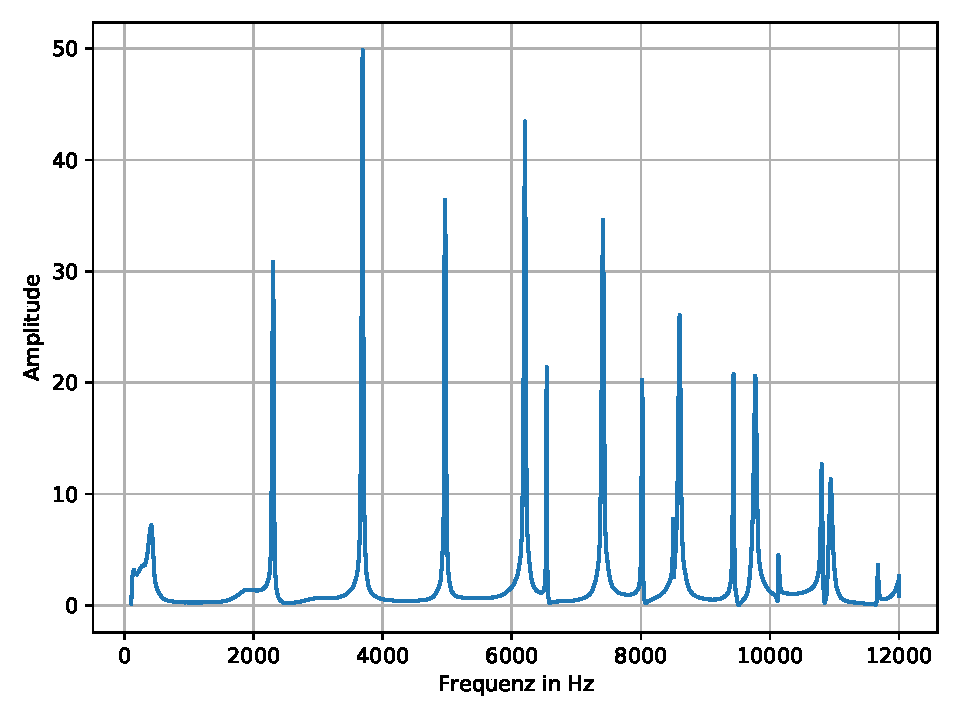
\includegraphics[width=0.75\textwidth]{pic/Wasserstoffatom.pdf}
    \caption{Hochauflösende Spektrum bei festen Winkel $\alpha=$180°}
    \label{fig:hf}
  \end{figure}

\noindent
Die danach händisch ermittelten Werte für die Resonanzfrequenzen $\nu_{Res}$ sind in der Tabelle (\ref{tab:1}) aufgeführt. Dabei fehlen für 2 Werte die Phasenverschiebungen
da diese bei der Messung vergessen wurden zu notieren.

\begin{table}[H]
    \center
    \caption{Resonanzfrequenz $\nu_{Res}$ mit zugehöriger Ordnung und Phasenverschiebung.}
    \label{tab:1}
    \begin{tabular}{l l l c}
        \toprule
        Ordnung & $\nu_{Res}\,/\,$kHz & $\varphi\,/\,°$\\
        \midrule
        1 &0,41   & -102  \\
        2 &2,288 &   70  \\
        3 &3,682 &  -78  \\
        4 &4,963 &   90  \\
        5 &6,203 &  -30  \\
        6 &6,595 &  k.A. \\
        7 &7,41 &  170  \\
        8 &8,018 &  -14  \\
        9 & 8,5 & k.A. \\
        10 &8,603 &   20  \\
        11 &9,437 & -150  \\
        12 &9,778 & -130  \\
        \bottomrule
    \end{tabular}
\end{table}

\subsubsection{Die Winkelabhängigkeit der Resonanzfrequenzen}

Die Winkelabhängigkeit der Resonanzfrequenzen bei ungefähr 2,288 kHz, 3,682 kHz, 4,963 kHz und 7,41 kHz werden zusätzlich untersucht und werden jeweils in der Form eines Polar Plot
dargestellt. Dieses ist in \autoref{fig:4} (orange eingezeichnet) zu finden.

\begin{figure}
    \centering
    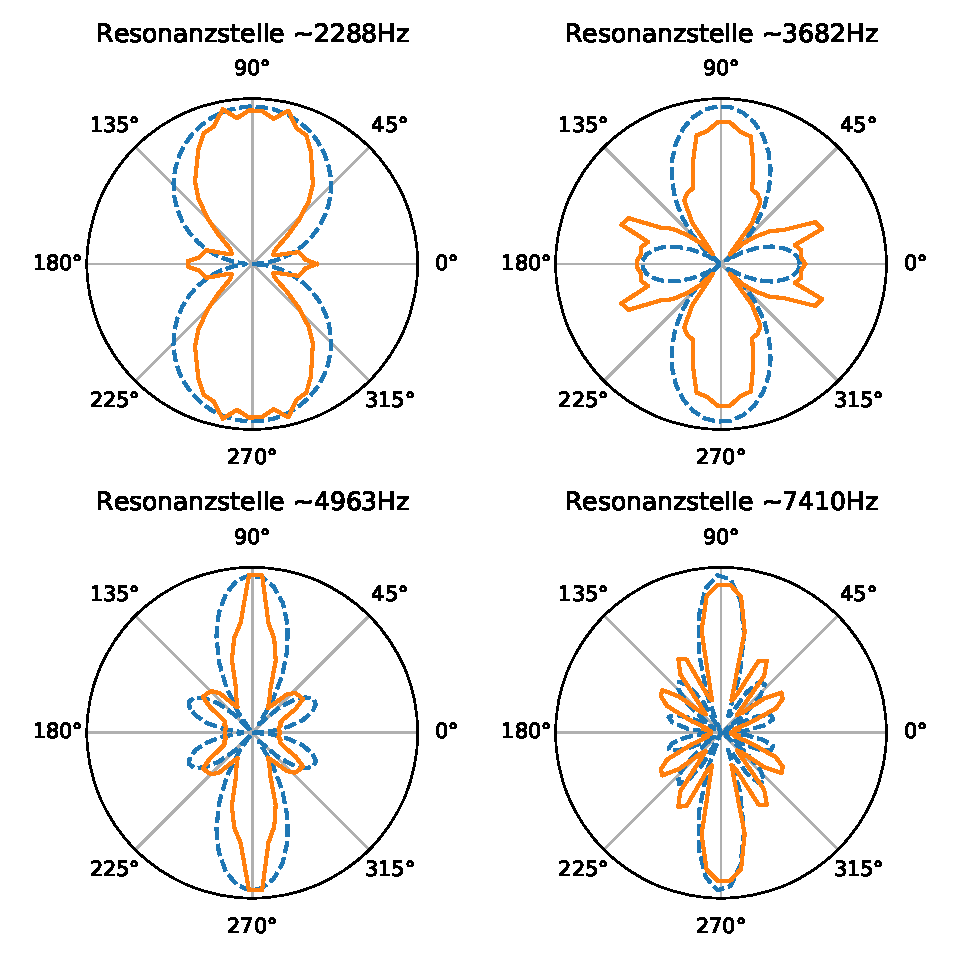
\includegraphics[width=0.75\textwidth]{pic/all.pdf}
    \caption{Untersuchte Resonanzstellen in einem Polarplot, mit dem Winkel gegen Amplitude aufgetragen}
    \label{fig:4}
  \end{figure}

Die Druckamplitude bei der Resonanzstelle ~ $2,288$kHz hat die Form eines $2{p}_0$-Orbitals, bei der Resonanzstelle ~ $3,682$kHz die Form eines $3{d}_0$-Orbitals,
bei der Resonanzstelle ~ $4,963$kHz die Form eines $4{f}_0$-Orbitals und bei der Resonanzstelle ~ $7,410$kHz die Form eines $6{h}_0$-Orbitals. Die theoretische Form
der Orbitale ist in der Skizze ebenfalls eingezeichnet (blau gestrichelt), wobei der Radius in allen Plots willkürlich gewählt ist.


\subsubsection{Aufspaltung der Zustände}
Um die Aufspaltung der Zustände im Wasserstoffatom nachzustellen, werden wie in \autoref{Wasserstoffatom} beschrieben Zwischenringe eingesetzt. Das diese Aufspaltung 
auch wirklich stattfindet wird exemplarisch in \autoref{fig:3mm} gezeigt.

\begin{figure}
    \centering
    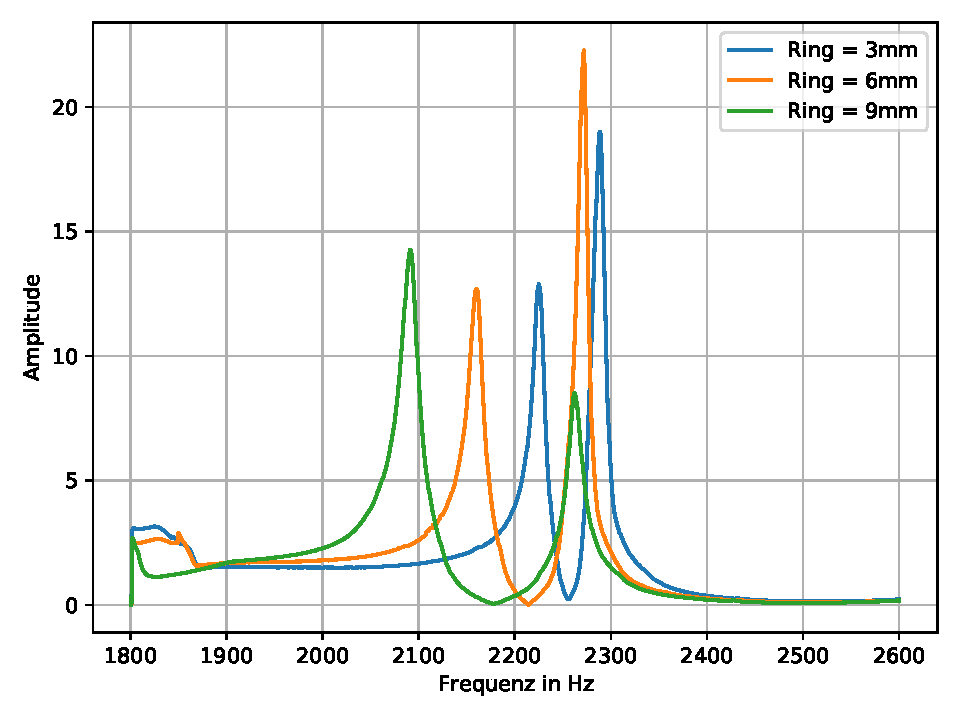
\includegraphics[width=0.75\textwidth]{pic/3mm.pdf}
    \caption{Aufspaltung der Resonanz bei ~ 2,3kHz in zwei Resonanzfrequenzen.}
    \label{fig:3mm}
  \end{figure}

  \noindent
  Wenn die Differenz der Resonanzfrequenzen je Ring gegen die Zwischenringbreite aufgetragen wird (\autoref{fig:aufspaltung}), so fällt auf, dass diese sich fast komplett linear zueinander verhalten.
  Das Analogon dieser Aufspaltung im Wasserstoffatom wäre der Zeemann-Effekt, welcher beim anlegen eines magnetischen Feldes zu beobachten ist.

\begin{figure}
  \centering
  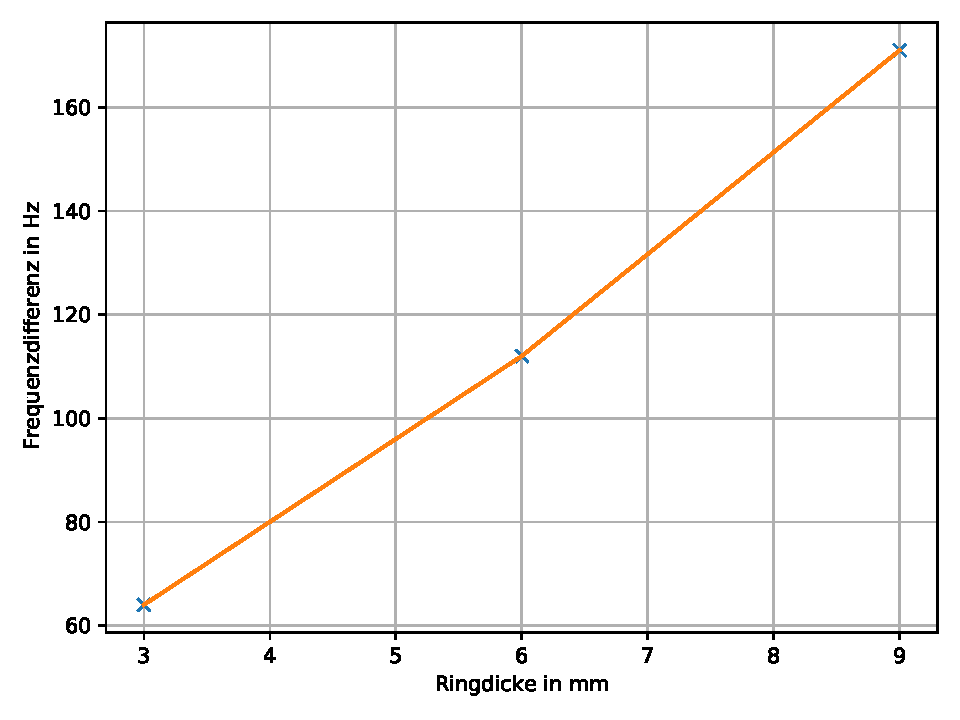
\includegraphics[width=0.75\textwidth]{pic/aufspaltung.pdf}
  \caption{Die Differenz der Resonanzfrequenz gegen die Ringbreite aufgetragen.}
  \label{fig:aufspaltung}
\end{figure}



\subsubsection{Zustandsaufspaltung und deren Winkelabhängigkeit}
Wie aus \autoref{fig:3mm} zu entnehmen ist, ist die Aufspaltung bei einem Zwischenring von 9mm am größten ($\alpha = $ 180°). Dabei stellt der erste Piek bei der einer
Resonanzfrequenz von 2091Hz im Model $m=0$ und $l=1$ und die Resonanzfrequenz 2262Hz im Model $m= \pm 1$ und $l=1$ dar.

\noindent
Die untersuchte Winkelverteilung ist in \autoref{fig:wink} zu finden und ist wieder in Form eines Polar Plots dargestellt.


\begin{figure}
    \centering
    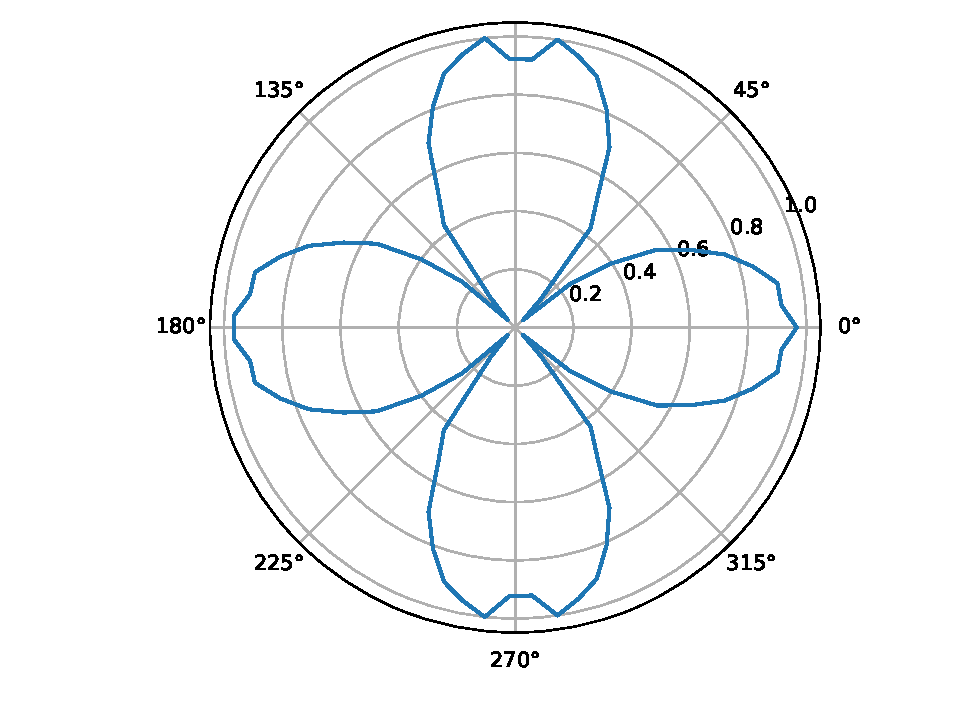
\includegraphics[width=0.75\textwidth]{pic/polar_9mm.pdf}
    \caption{Die Differenz der Resonanzfrequenz gegen die Ringbreite aufgetragen.}
    \label{fig:wink}
  \end{figure}
  
\subsection{Wasserstoffmolekül}
Mithilfe des zusätzlich eingesetzten Kugelresonators kann ein Wasserstoffmolekül nachgestellt werden. Durch die unterschiedlich großen Blenden werden unterschiedlich
starke Kopplungen nachgestellt. Dies kann in \autoref{fig:kop} gesehen werden. 

\begin{figure}
    \centering
    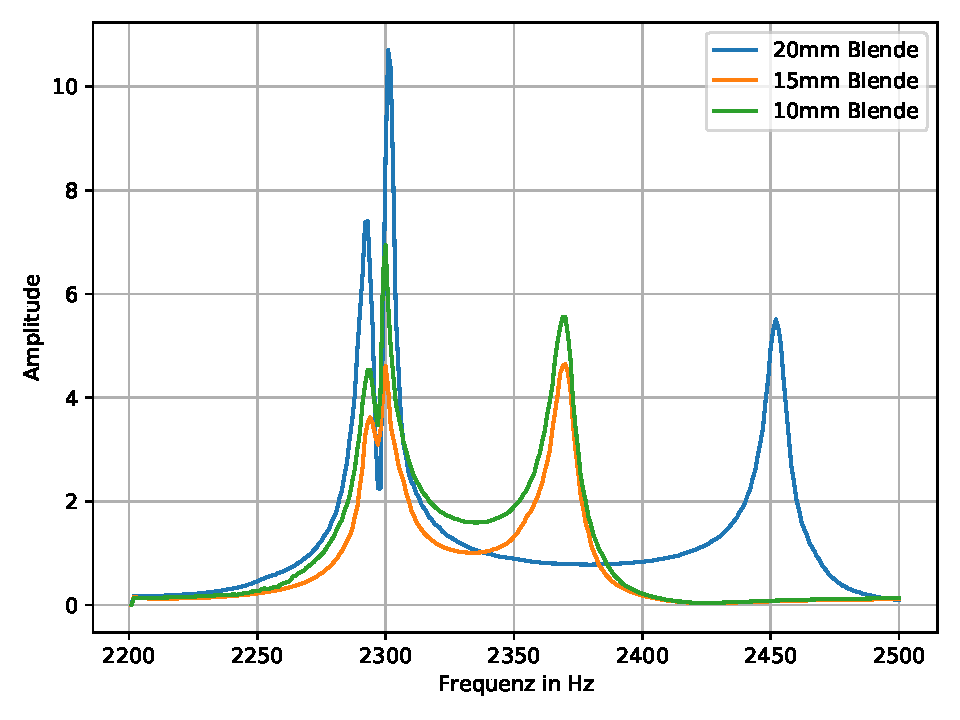
\includegraphics[width=0.75\textwidth]{pic/101520.pdf}
    \caption{Frequenzspektrum bei unterschiedlich großen Blenden gegen die Amplitude aufgetragen.}
    \label{fig:kop}
  \end{figure}

\noindent
Beobachtet werden jeweils 3 Resonanzfrequenzen. Bei der 15mm Blende  werden diese in Abhängigkeit gemessen und gegenüber dem Winkel in \autoref{fig:polar3} aufgetragen. Die Phasenverschiebung ist in 
\autoref{tab:phasen} zu finden.

\begin{figure}
    \label{fig:polar3}
    \centering
    \begin{subfigure}[b]{0.3\textwidth}
        \centering
        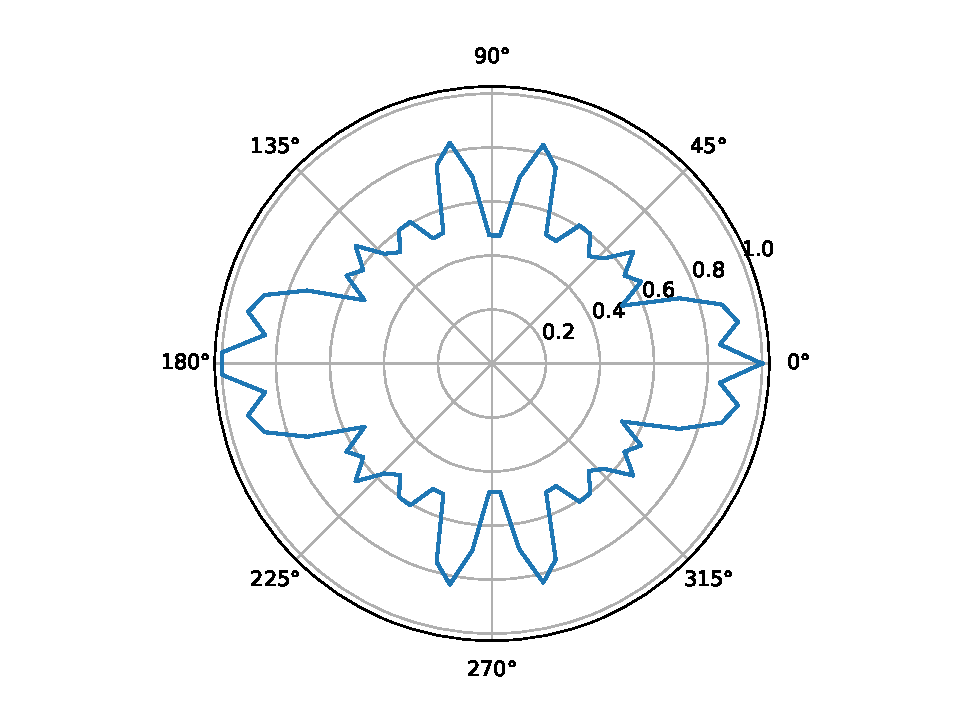
\includegraphics[width=\textwidth]{pic/polar_max_294.pdf}
        \caption{Resonanzfrequenz 2294Hz}
    \end{subfigure}
    \hfill
    \begin{subfigure}[b]{0.3\textwidth}
        \centering
        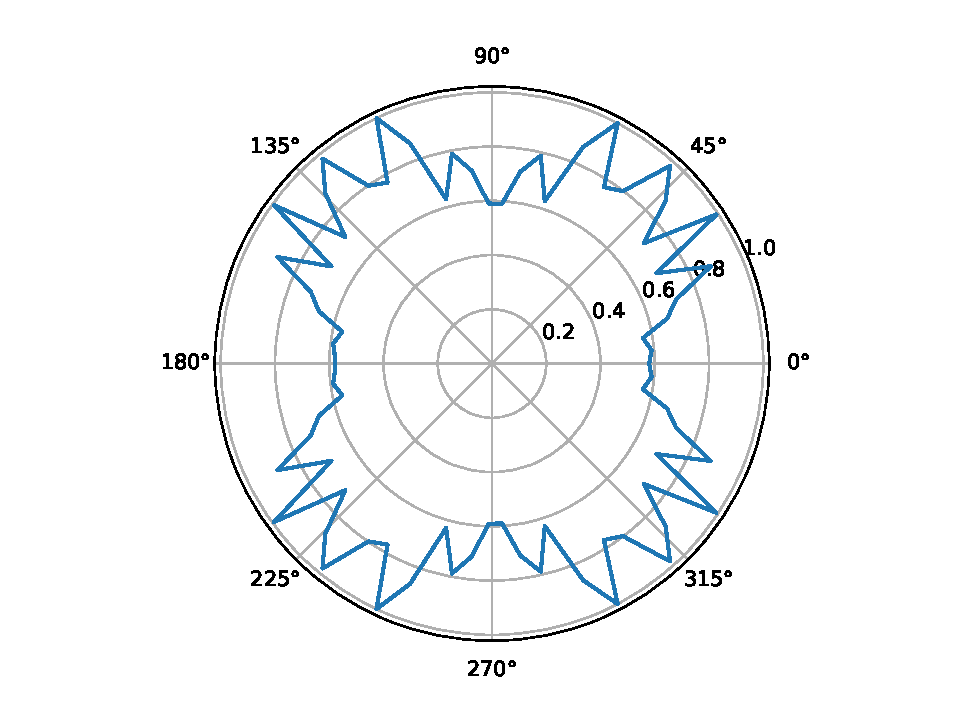
\includegraphics[width=\textwidth]{pic/polar_max_298.pdf}
        \caption{Resonanzfrequenz 2298Hz}
    \end{subfigure}
    \hfill
    \begin{subfigure}[b]{0.3\textwidth}
        \centering
        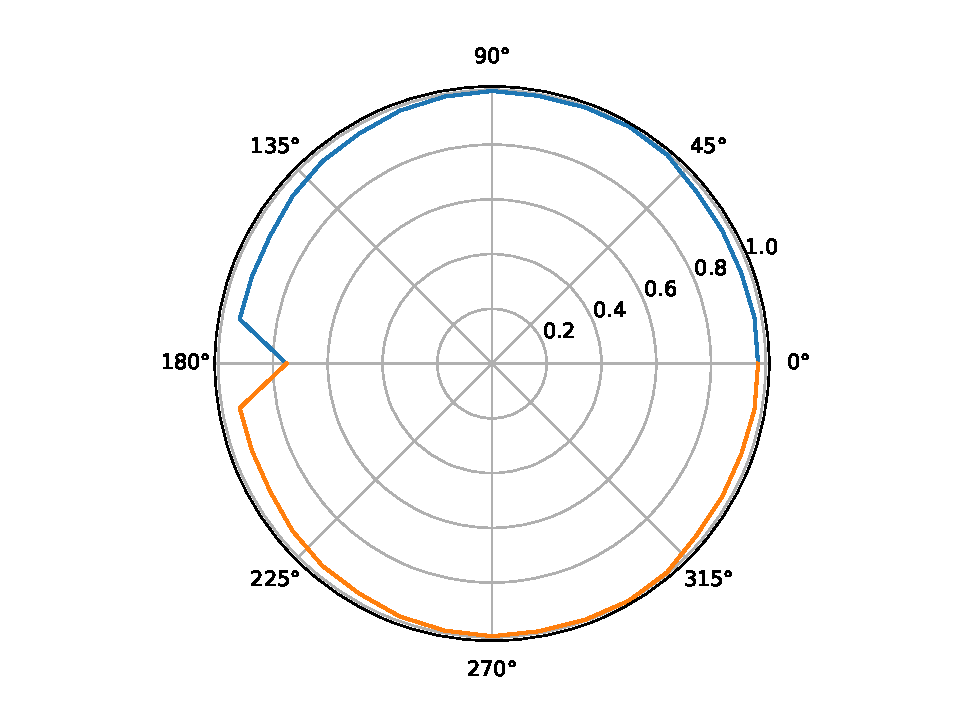
\includegraphics[width=\textwidth]{pic/polar_max_369.pdf}
        \caption{Resonanzfrequenz 2370Hz}
    \end{subfigure}
    \caption{Polar Plots der 3 Resonanzfrequenzen bei der 15mm Blende}
\end{figure}

\begin{table}
    \caption{}
    \center
    \begin{tabular}{c| c c c c}
        \toprule
        Ordnung & $\nu_{Res}\,/\,$kHz & obere Phasendiff. $\,/\,°$ & untere Phasendiff. $\,/\,°$ & $\Delta$ Phasendiff. $\,/\,°$\\
        \midrule
        1 &2,294 &-145 &-51 &196 \\
        2 &2,298 &-135 &23,5 & 111,5\\
        3 &2,370 &-32 &138 & 106\\
        \bottomrule
    \end{tabular}
    \label{tab:phasen}
\end{table}


\subsection{eindimensionaler Festkörper}
Eine 'Kette' an Resonatoren kann genutzt werden um einen 1-dim Festkörper genähert darzustellen. Dabei wird wie in \autoref{fkp} erläutert zunächst 2 Zylinder
mit einer 16mm Blende dazwischen, dann 4 und dann 10 Zylinder mit jeweils einer 16mm Blende zwischen den Zylindern aufgebaut und in einem Frequenzspektrum durchgemessen.
Die Frequenzspektren sind in der \autoref{fig:16mm} zu sehen.

\noindent
Was dabei auffällt ist, dass sich Gruppen an Maxima bilden, wobei jedes Maxima in einer Gruppe für ein Zylinder steht. Auf den Festkörper übertragen würde jeder 
Zylinder für ein Band steht und wenn mehr Zylinder hinzugefügt werden auch mehr Bänder entstehen, auf denen sich die elektronen aufhalten können.

\noindent
Die Freiräume zwischen den Gruppen wären dann die sogenannten Bandlücken, also stellen, an denen sich die Elektronen nicht aufhalten können.

\begin{figure}[H]
    \centering
    \subfloat[Frequenzspektrum für eine Resonatorkette aus zwei Resonatorgliedern (Rohrzylindern) mit einer jeweiligen Länge von $50$mm und einer $16$mm-Blende als Zwischenstück.]{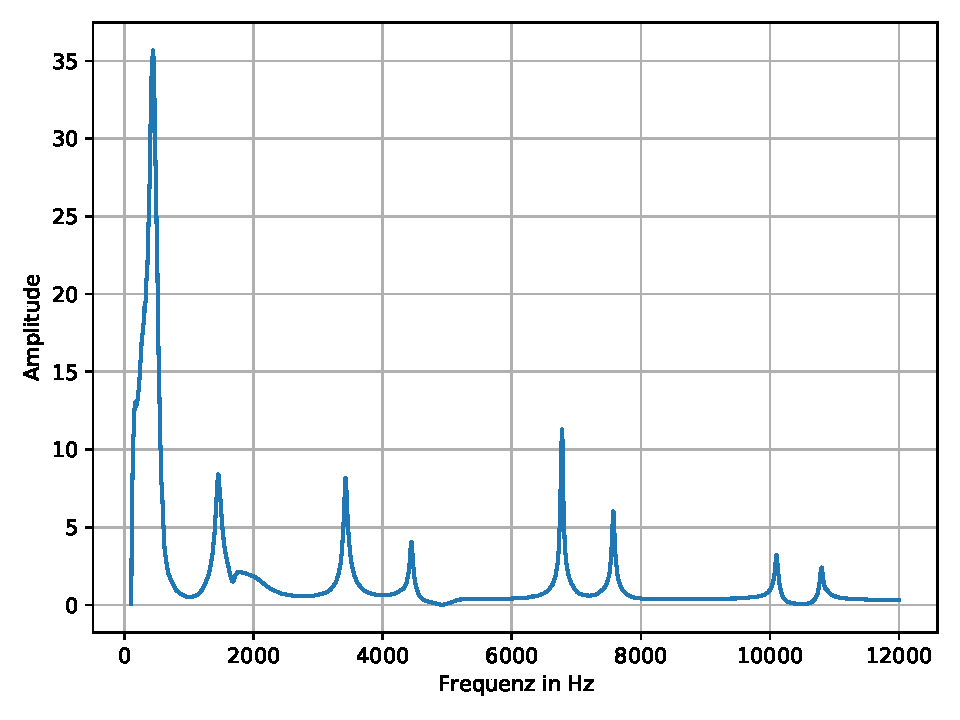
\includegraphics[width=0.45\textwidth]{pic/festkoerper_16mm/2_16.pdf}}\hfil
    \subfloat[Frequenzspektrum für eine Resonatorkette aus vier Resonatorgliedern (Rohrzylindern) mit einer jeweiligen Länge von $50$mm und einer $16$mm-Blende als Zwischenstück.]{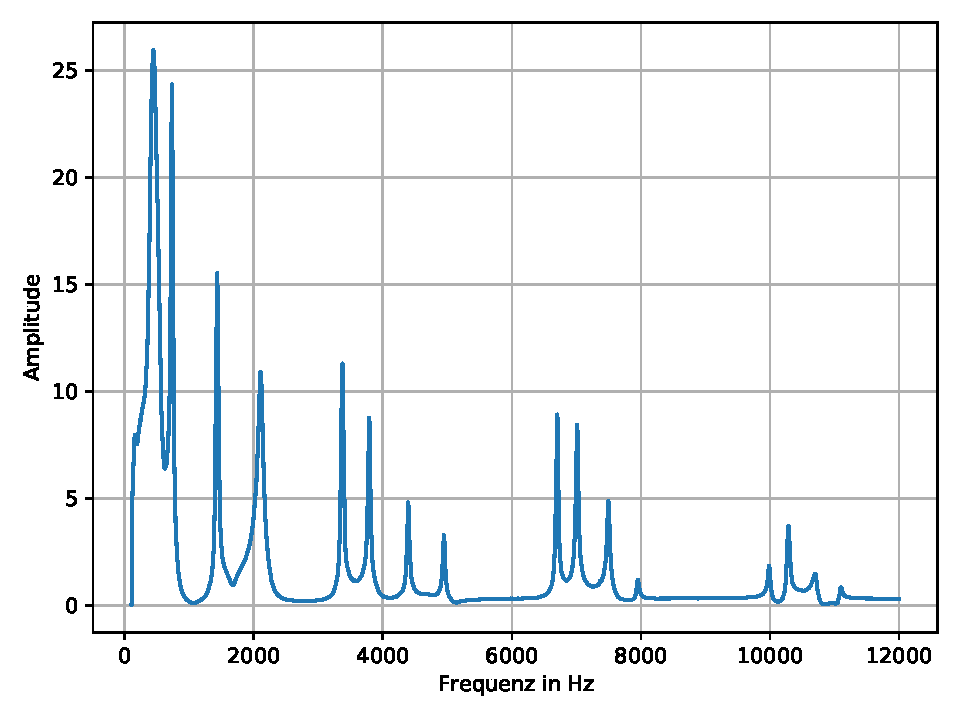
\includegraphics[width=0.45\textwidth]{pic/festkoerper_16mm/4_16.pdf}}\hfil 
    
    \subfloat[Frequenzspektrum für eine Resonatorkette aus zehn Resonatorgliedern (Rohrzylindern) mit einer jeweiligen Länge von $50$mm und einer $16$mm-Blende als Zwischenstück..]{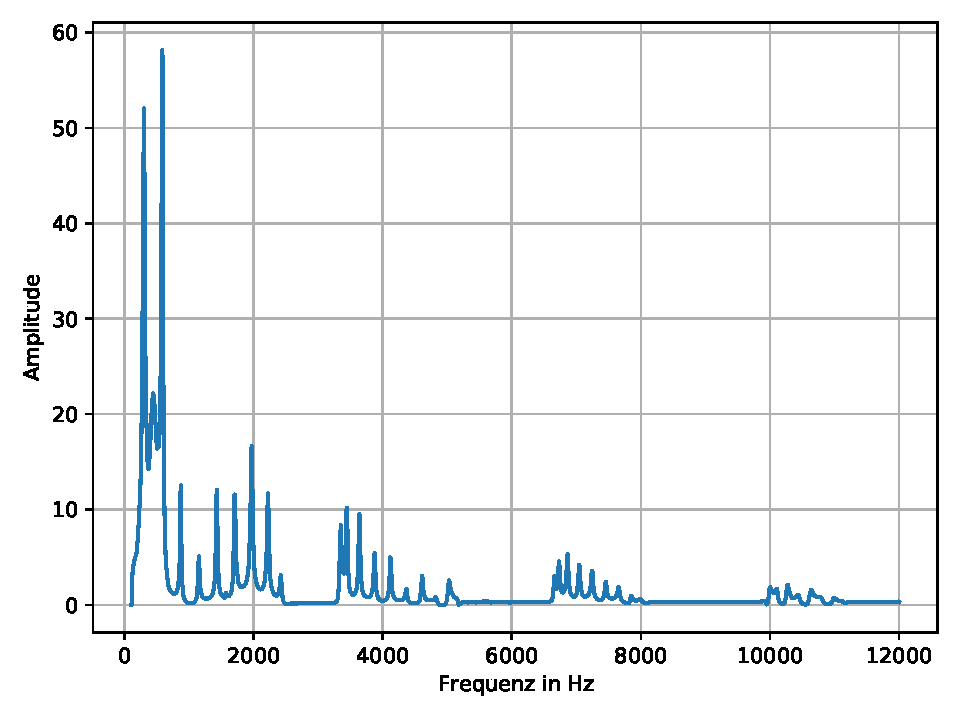
\includegraphics[width=0.45\textwidth]{pic/festkoerper_16mm/10_16.pdf}}\hfil
    \caption{}
    \label{fig:16mm}
\end{figure}

\noindent
Das gleiche kann ebenfalls mit Blenden aufgebaut werden, mit einem kleineren Durchmesser, sodass folgende Frequenzspektrum \ref{fig:10mm}, \ref{fig:13mm} entstehen.

\begin{figure}[H]
    \centering
    \subfloat[Frequenzspektrum für eine Resonatorkette aus zwei Resonatorgliedern (Rohrzylindern) mit einer jeweiligen Länge von $50$mm und einer $13$mm-Blende als Zwischenstück.]{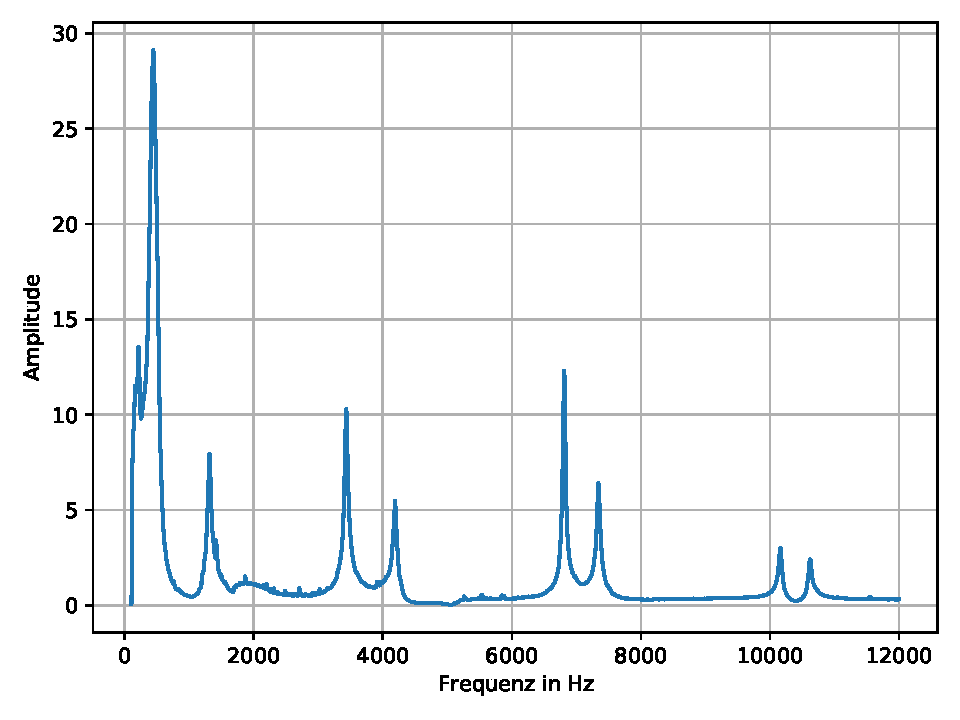
\includegraphics[width=0.45\textwidth]{pic/festkoerper_13mm/2_13.pdf}}\hfil
    \subfloat[Frequenzspektrum für eine Resonatorkette aus vier Resonatorgliedern (Rohrzylindern) mit einer jeweiligen Länge von $50$mm und einer $13$mm-Blende als Zwischenstück.]{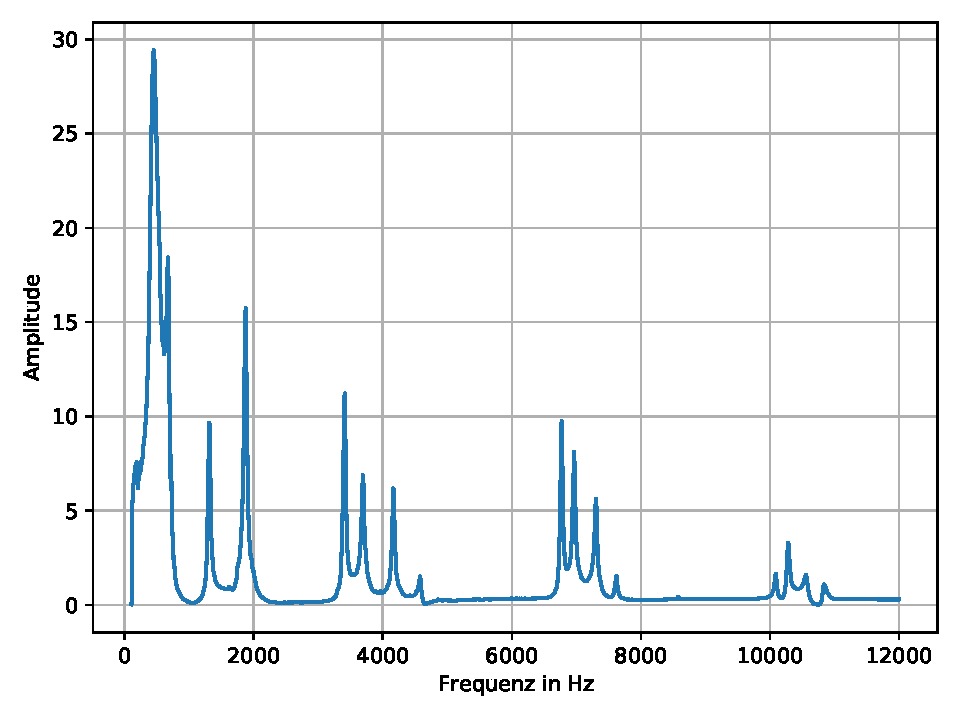
\includegraphics[width=0.45\textwidth]{pic/festkoerper_13mm/4_13.pdf}}\hfil 
    
    \subfloat[Frequenzspektrum für eine Resonatorkette aus zehn Resonatorgliedern (Rohrzylindern) mit einer jeweiligen Länge von $50$mm und einer $13$mm-Blende als Zwischenstück..]{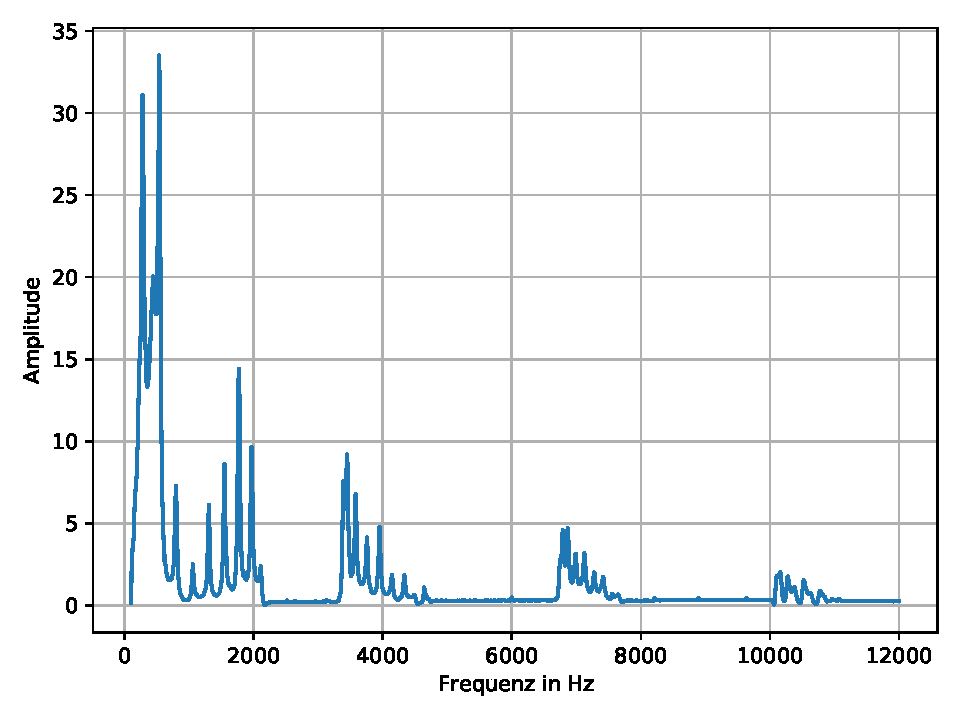
\includegraphics[width=0.45\textwidth]{pic/festkoerper_13mm/10_13.pdf}}\hfil
    \caption{}
    \label{fig:13mm}
\end{figure}

\begin{figure}[H]
    \centering
    \subfloat[Frequenzspektrum für eine Resonatorkette aus zwei Resonatorgliedern (Rohrzylindern) mit einer jeweiligen Länge von $50$mm und einer $10$mm-Blende als Zwischenstück.]{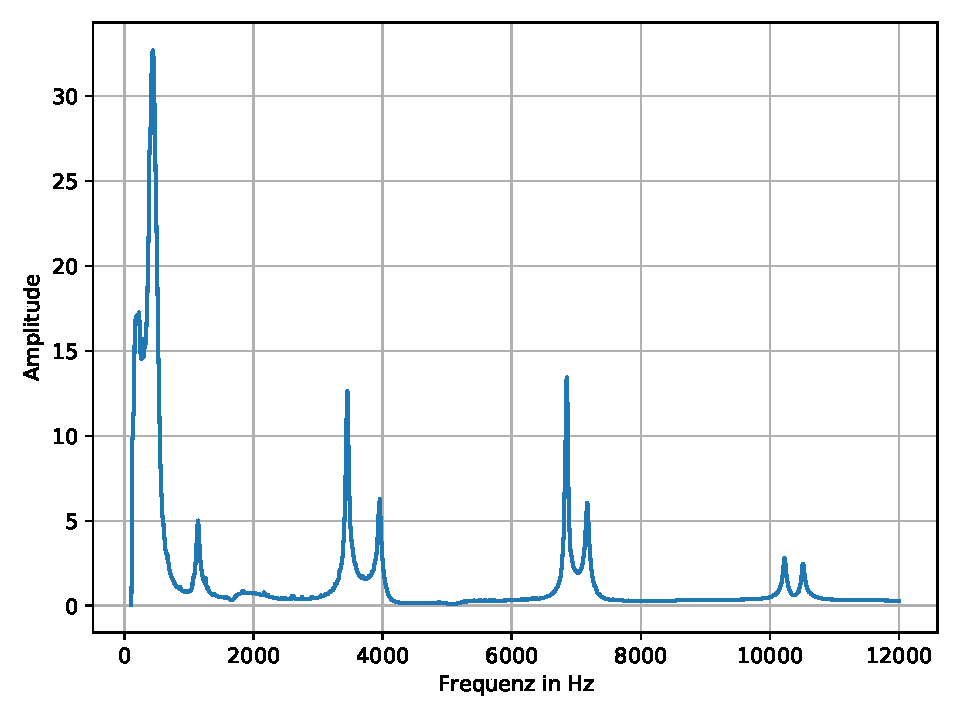
\includegraphics[width=0.45\textwidth]{pic/festkoerper_10mm/2_10.pdf}}\hfil
    \subfloat[Frequenzspektrum für eine Resonatorkette aus vier Resonatorgliedern (Rohrzylindern) mit einer jeweiligen Länge von $50$mm und einer $10$mm-Blende als Zwischenstück.]{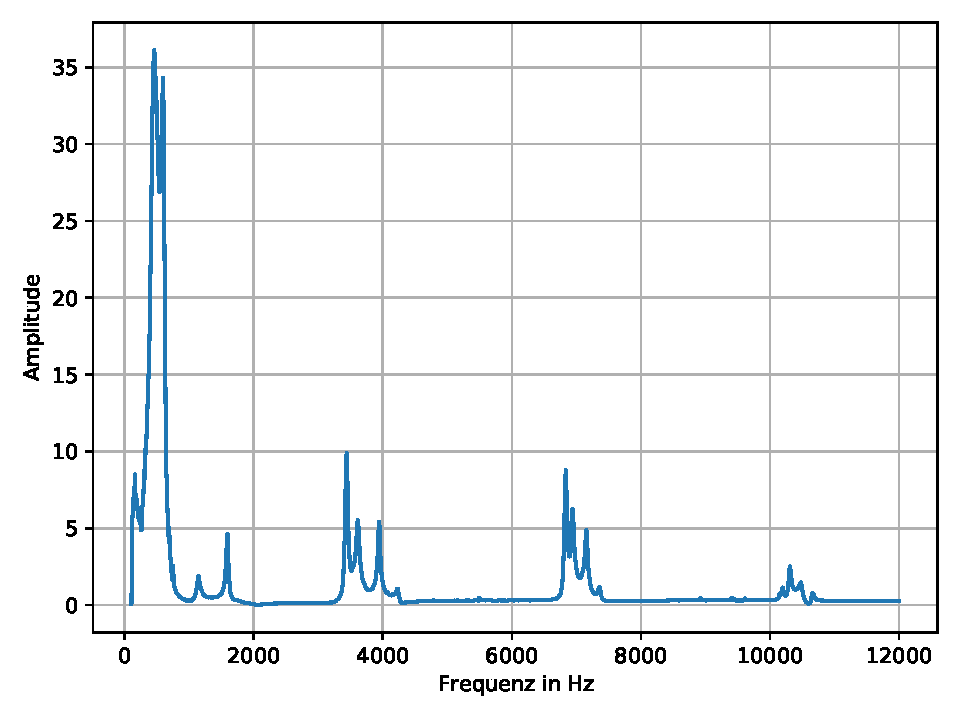
\includegraphics[width=0.45\textwidth]{pic/festkoerper_10mm/4_10.pdf}}\hfil 
    
    \subfloat[Frequenzspektrum für eine Resonatorkette aus zehn Resonatorgliedern (Rohrzylindern) mit einer jeweiligen Länge von $50$mm und einer $10$mm-Blende als Zwischenstück..]{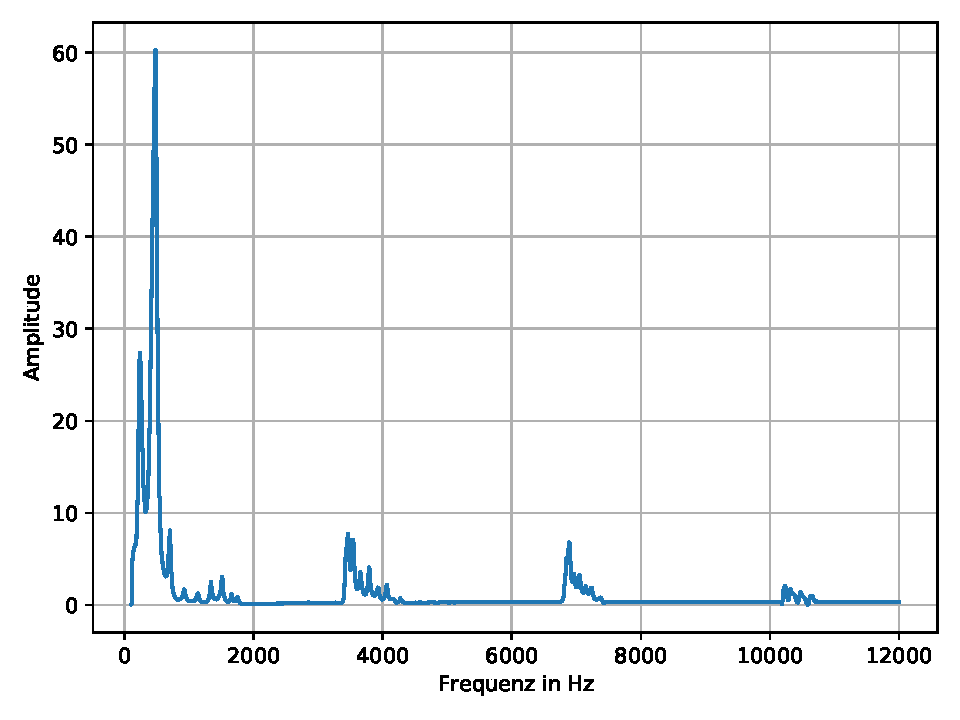
\includegraphics[width=0.45\textwidth]{pic/festkoerper_10mm/10_10.pdf}}\hfil
    \caption{}
    \label{fig:10mm}
\end{figure}

\noindent
Auffällig dabei ist, dass umso kleiner der Durchmesser der Blende ist, desto höher sind die Maxima.


\subsubsection{Störstellen im Festkörper}
Es können mit diesem Modell ebenfalls Störstellen im Kristall nachgestellt werden, durch die Variation der länger der Zylinder. In diesem fall wurde ein Zylinder der Länge
von 50mm gegen ein 37,5mm, 62,5mm und ein 75mm langen Zylidner ausgetauscht und wieder mit dem gleichen Frequenzspektren abgefahren. Dies kann in \autoref{fig:stoer} gesehen werden.

\begin{figure}[H]
    \centering
    \subfloat[Fehlstelle mit $37,5$mm Zylinder.]{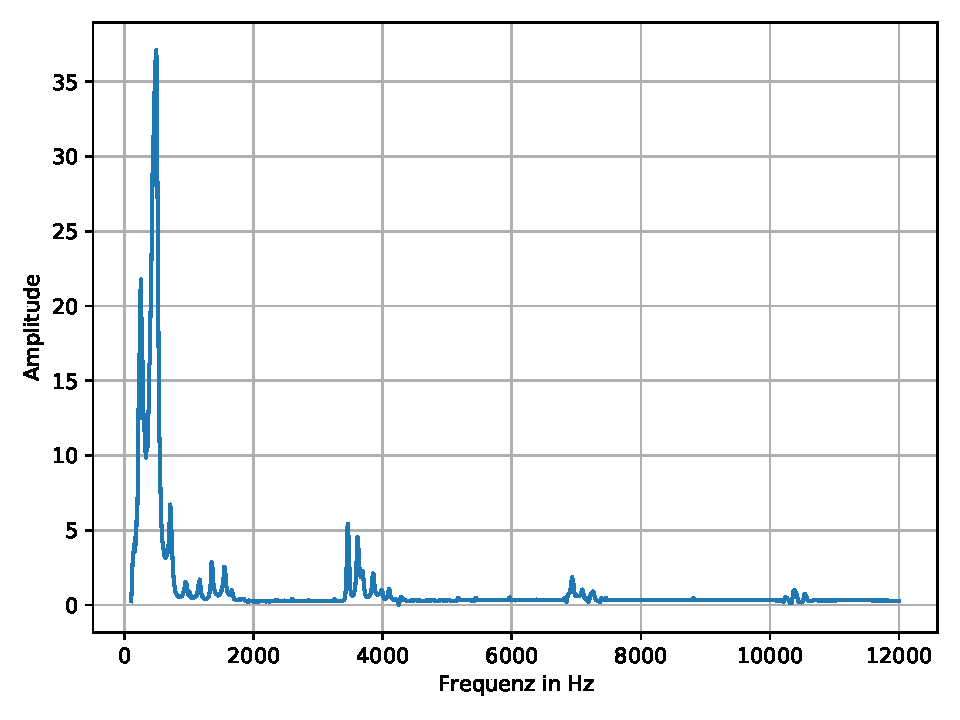
\includegraphics[width=0.45\textwidth]{pic/festkoerper_stoerstelle/37,5mm.pdf}}\hfil
    \subfloat[Fehlstelle mit $62,5$mm Zylinder.]{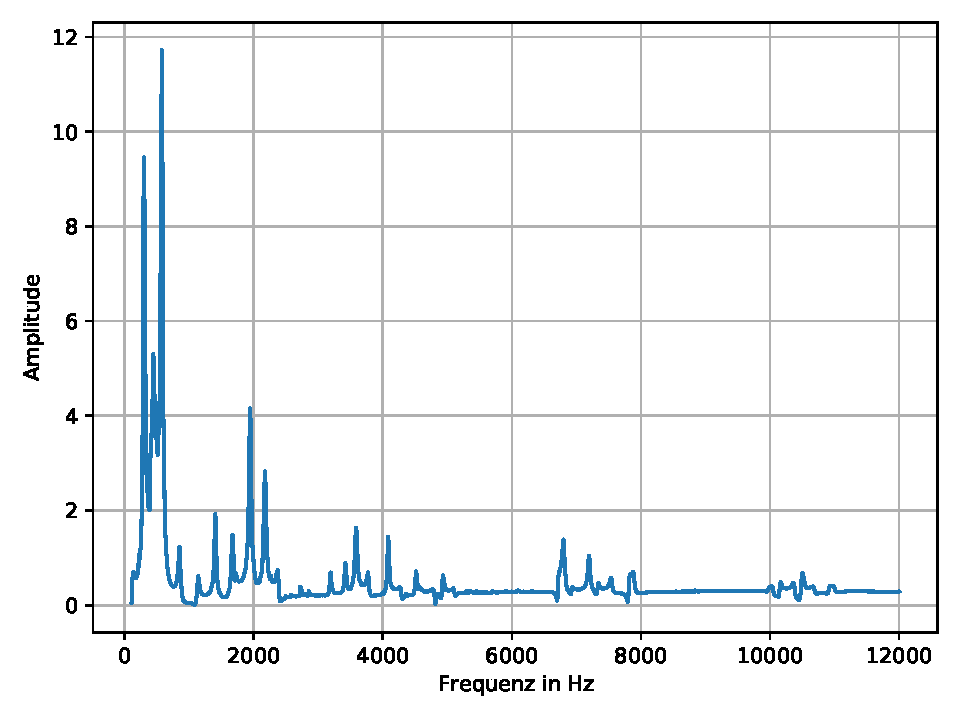
\includegraphics[width=0.45\textwidth]{pic/festkoerper_stoerstelle/62,5mm.pdf}}\hfil 
    \subfloat[Fehlstelle mit $75$mm Zylinder.]{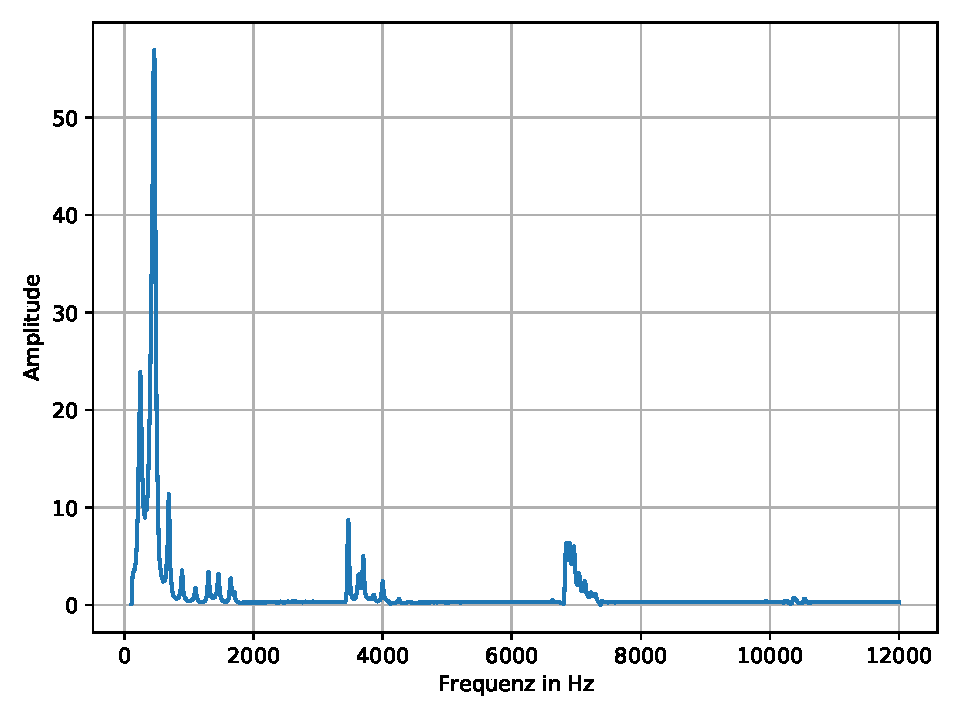
\includegraphics[width=0.45\textwidth]  {pic/festkoerper_stoerstelle/75mm.pdf}} 
    \caption{Frequenzspektren für eine Resonatorkette aus neun Zylindern der Länge $50\,$mm und einer Störstelle durch einen Zylinder einer anderen Länge. Zwischenstücke bilden $10\,$mm Blenden.}
    \label{fig:fest_stoer}
\end{figure}

\noindent
Es ist im Vergleich zum ungestörten Festkörper eine neue Resonanz in der Gruppe zu beobachten, dessen Maxima das der Gruppe deutlich übersteigt.

\subsubsection{abwechselnden Zylinderlängen}
Um einen Festkörper, welcher aus 2 unterschiedlichen Elementen besteht nachzustellen, wie z.B. eine GaAs-Kristall, wird abwechselnd ein 50mm und ein 75mm langer Zylinder
mit jeweils einer 16mm Blende dazwischen verbaut und wieder im gleichen Frequenzspektrum durchgemessen. Das Spektrum kann in \autoref{fig:abwech_zylin} betrachtet werden.

\begin{figure}[H]
    \centering
    \subfloat[Frequenzspektrum eines einzelnen Zylinders mit der Länge von $75\,$mm.]{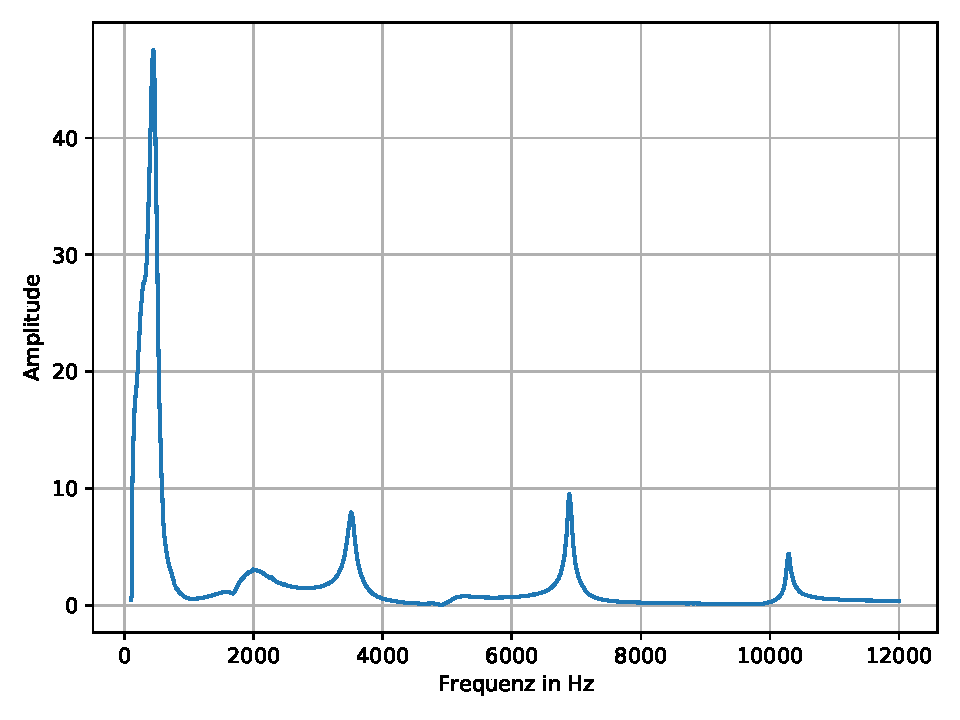
\includegraphics[width=0.45\textwidth]{pic/nur50.pdf}}\hfil 
    \subfloat[Frequenzspektrum eines einzelnen Zylinders mit der Länge von $50\,$mm.]{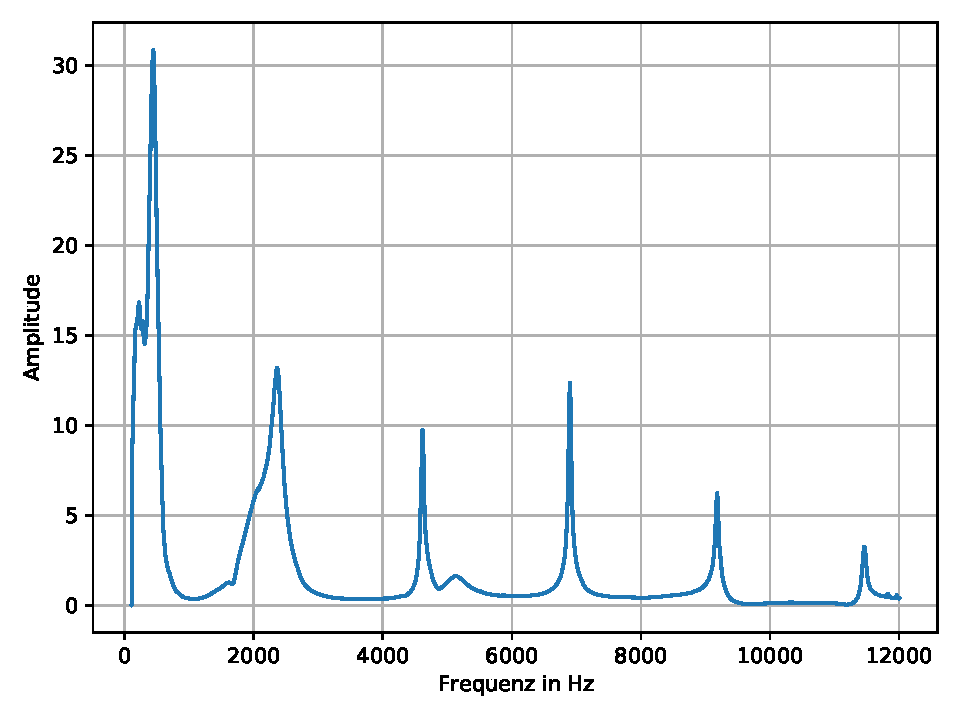
\includegraphics[width=0.45\textwidth]{pic/nur75.pdf}}\hfil 
    \subfloat[Frequenzspektrum einer Resonatorkette mit zehn wechselden Zylindern der Länge $50\,$mm und $75\,$mm und Blenden mit einem Durchmesser von $16\,$mm.]{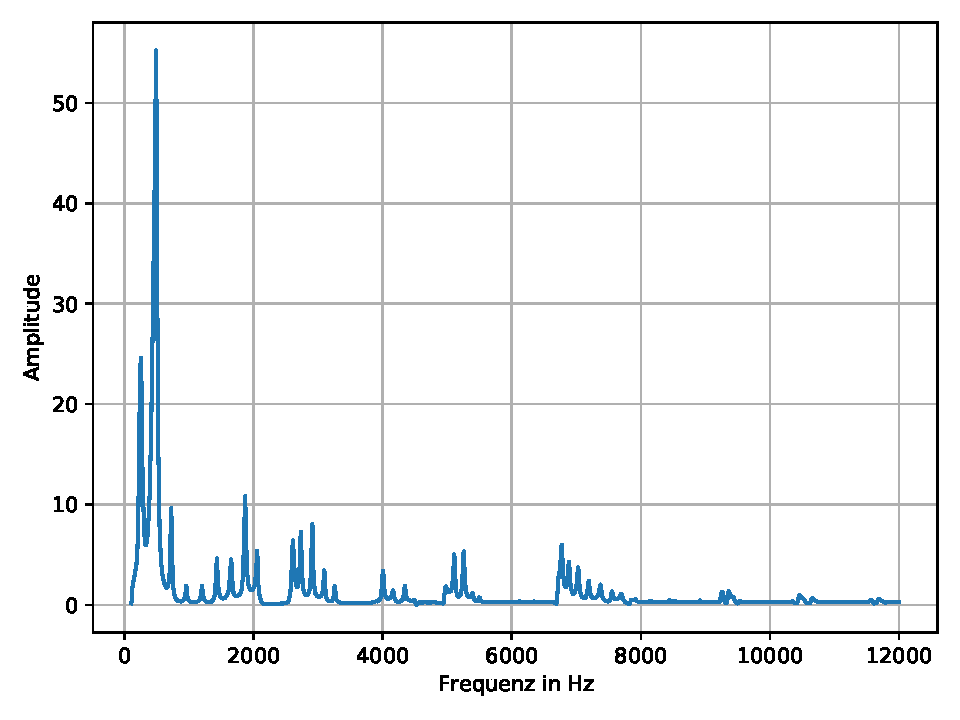
\includegraphics[width=0.8\textwidth]{pic/abwechselnd50u75.pdf}} 
    \caption{}
    \label{fig:abwech_zylin}
\end{figure}

\noindent
In der Sprache der Festkörperphysik ausgedrückt kann der \autoref{fig:abwech_zylin} entnommen werden, dass die Resonanzen der einzelnen ein-atomigen Basen in 
die zwei-atomigen-basen übernommen werden.

\subsubsection{Resonatorkette mit wechselndem Blendendurchmesser}
Nun kann ebenfalls wie zuvor der Blendendurchmesser variiert werden. Dies passiert durch das abwechseln einer 13mm Blende(3mal verbaut) mit einer 16mm Blende (4mal verbaut), sodass 
nun eine in \autoref{fig:abwech_blende} übergeordnete Periodizität beobachtet werden kann.

\begin{figure}
    \center
    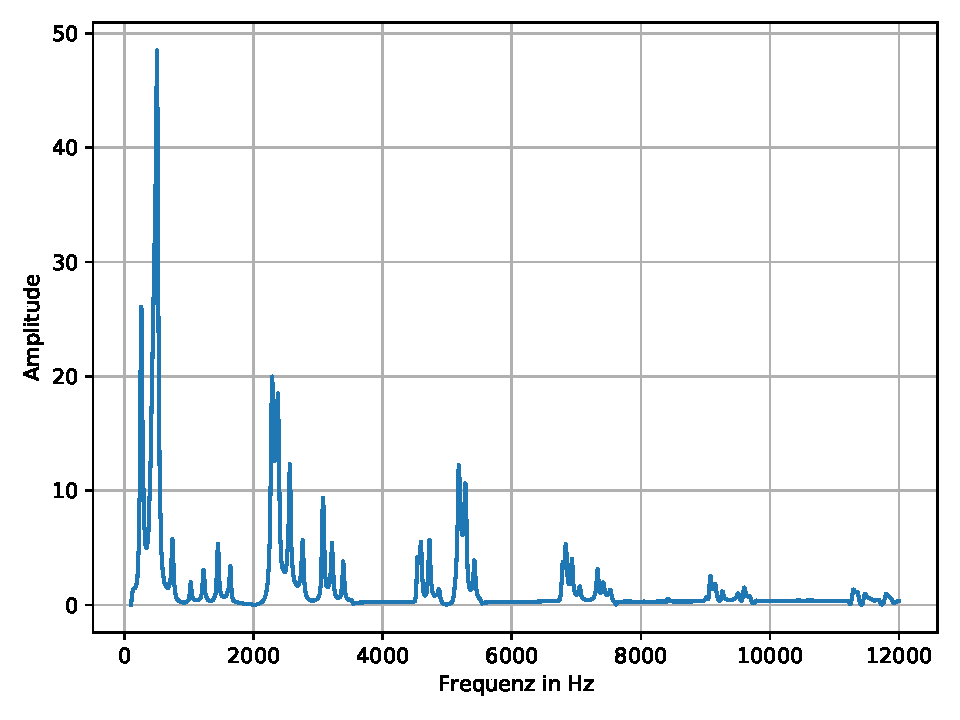
\includegraphics[width=0.8\textwidth]{pic/13u16.pdf}
    \caption{Frequenzspektrum einer Resonatorkette aus acht $75\,$mm langen Zylindern, welche abwechselnd durch $13$mm und $16$mm-Blenden getrennt sind.}
    \label{fig:abwech_blende}
\end{figure}
